
\marginpar{\href{https://youtu.be/TluTv5V0RmE}{Video}} Read sections: 1.3, 1.4\\
\marginpar{\href{https://ocw.mit.edu/courses/6-041sc-probabilistic-systems-analysis-and-applied-probability-fall-2013/pages/unit-i/lecture-2/}{Lecture Home}}
\marginpar{\href{https://ocw.mit.edu/courses/6-041sc-probabilistic-systems-analysis-and-applied-probability-fall-2013/a1462fa23de9d08c0dfd233a57278fed_MIT6_041SCF13_L02.pdf}{Slides}}

Example where countability axiom does not apply: We are not dealing with a \textit{sequence of sets}.

Zero probability doesn't mean impossible, just extremely unlikely by itself.

Expect the unexpected (10m)

$P(X)=1$ also doesn't mean certain.  "Essential certainty"

The issue is with continuous models.

\subsection{Conditional Probabilities}

\begin{figure}[ht]
\centering
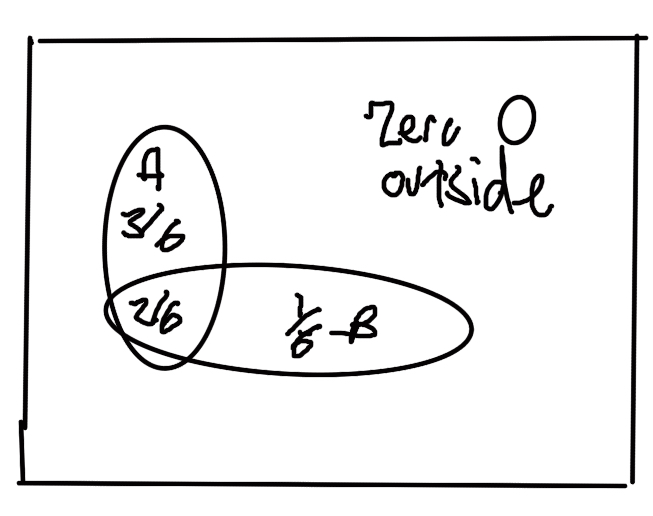
\includegraphics[width=10cm, height=7cm]{images/L02/cond_prob.jpeg}
\caption{Conditional Probabilities}
\end{figure}

$\frac{2}{6}$ is twice as likely as $\frac{1}{6}$. Want to keep proportion (16m)

$P(A|B)=$ Probability of A, given that B occurred.  B is our new universe.

\subsubsection{Definition}

\begin{align}
P(A|B) = \frac{P(A \cap B)}{P(B)}, \qquad \text{Assuming} P(B) \ne 0  
\end{align}
\myequations{Conditional Probability}

$$
\frac{2/6}{3/6} = \frac{2}{3}
$$

\marginpar{(17:30)} Can rewrite:
$$
P(A \cap B) = P(A \mid B)P(B) = P(B \mid A)P(A), \text{symmetrical relationship} 
$$

\marginpar{(19m)} These conditional probabilities are just probabilities and satisfy axioms.

\begin{align*}
A \cap B = \varnothing\\
P(A \cup B) = P(A) + P(B)
\end{align*}

Now we are placed in a universe where C occurred.

\begin{align*}
P(A \cup B \mid C) = P(A \mid C) + P(B \mid C)
\end{align*}

\subsection{Example: Dice Roll}

\marginpar{(23m)} The shortcut answer: Start with Uniform distribution, still uniform after we condition.

\begin{figure}[!ht]
\centering
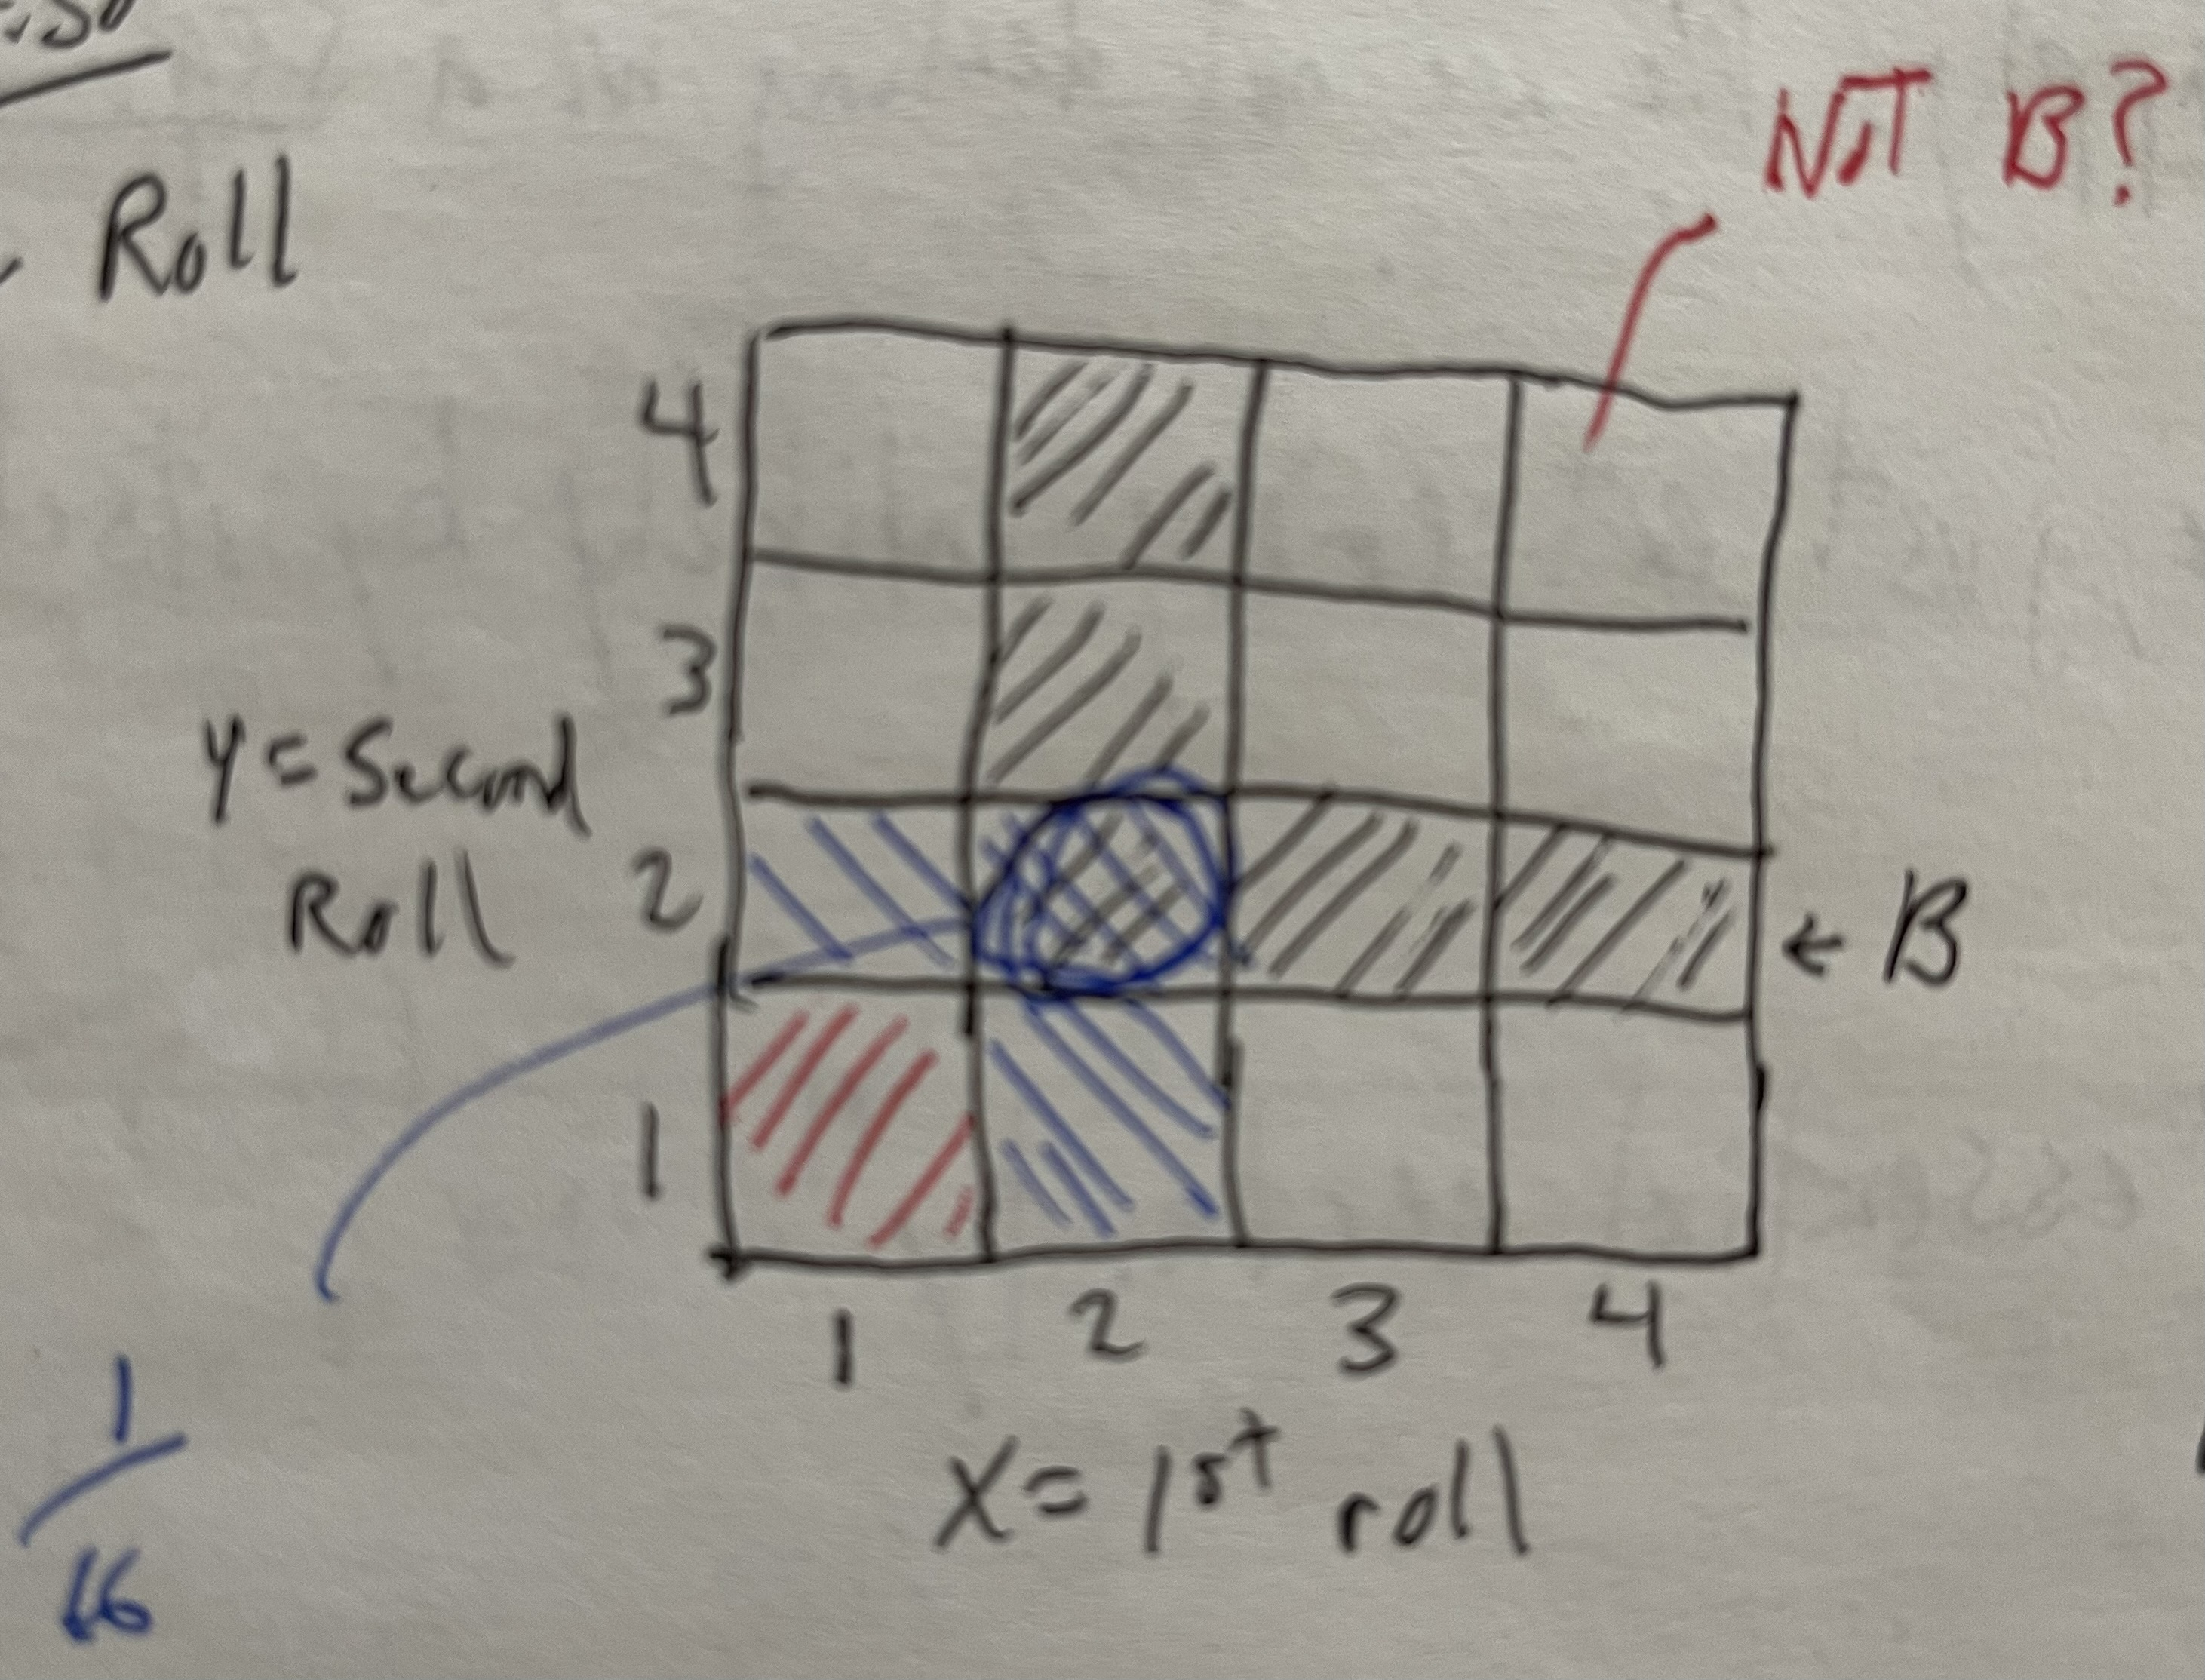
\includegraphics[width=6cm, height=4cm]{images/L02/dice_roll.jpeg}
\caption{Sample Space: Roll 2 Die}
\end{figure}

\subsection{Example: Airplane}

\marginpar{(24:45)}

\begin{itemize}
    \item Event A: Airplane is flying above
    \item Event B: Something registers on the radar screen
\end{itemize}

\begin{figure}[ht]
\centering
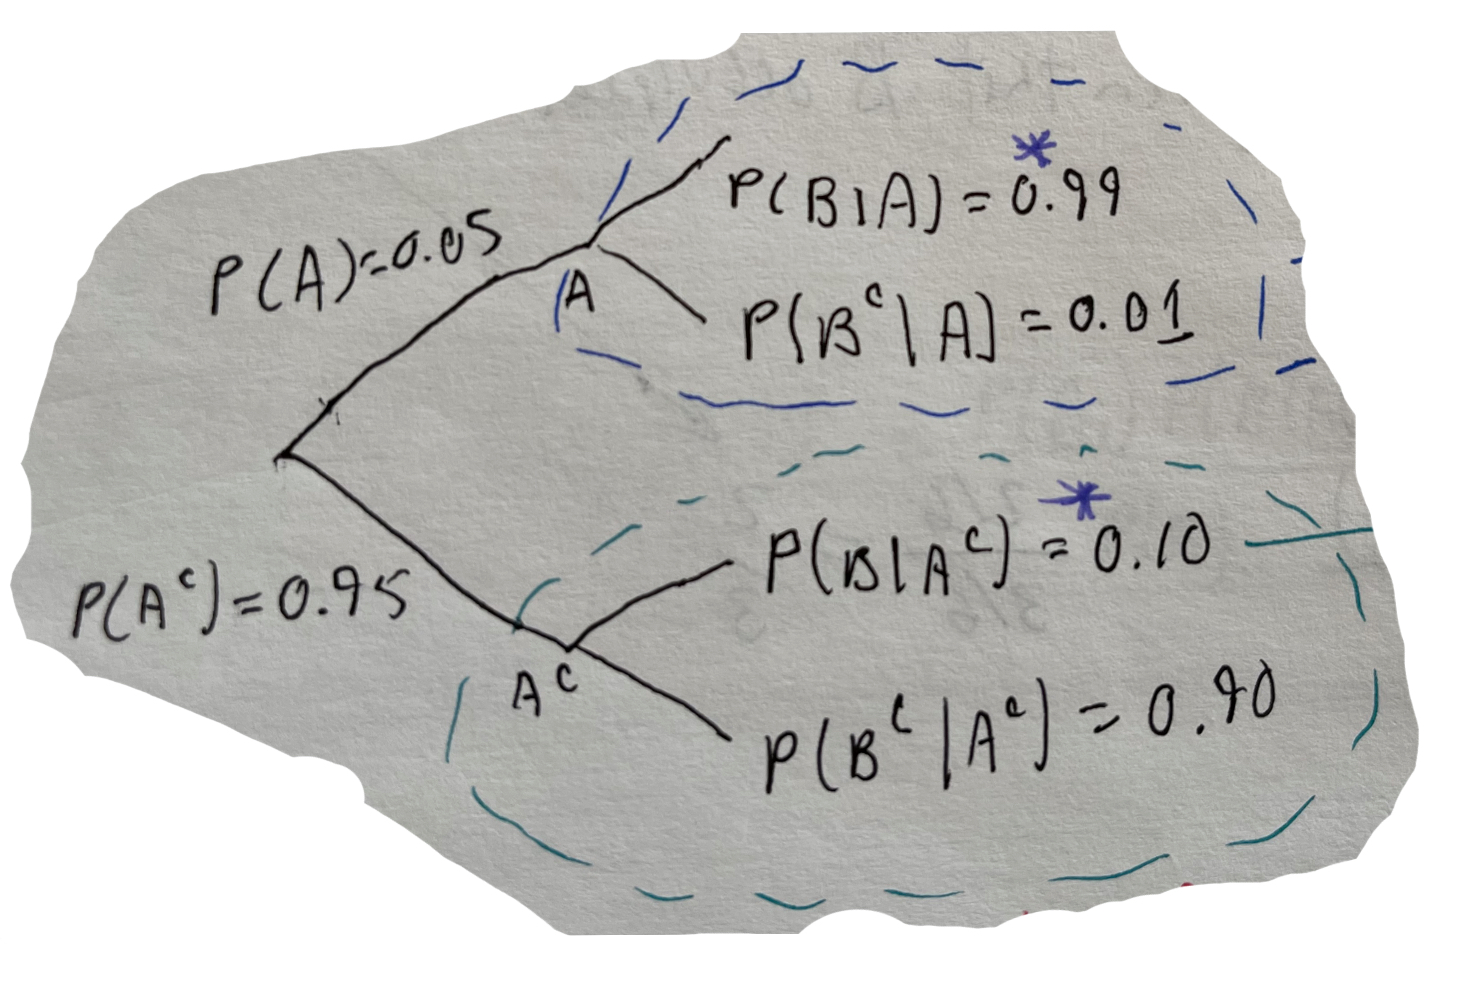
\includegraphics[width=5cm, height=4cm]{images/L02/airplane_radar.jpeg}
\caption{Airplane Probabilities}
\end{figure}

Can we derive ordinary probabilities starting from conditional?

\begin{align*}
P(A \cap B) = P(A)P(B|A) = 0.05\cdot 0.99 = 0.0495\\
P(B) =\\
P(A|B) =\\
\end{align*}

\marginpar{(28:25)}

What's the probability that our radar registers something? $P(B)$

\subsection{Multiplication Rule}

\marginpar{(34m)}

Multiply branches


\subsection{Total Probability Theorem}

Partition sample space.

\begin{figure}[ht]
\centering
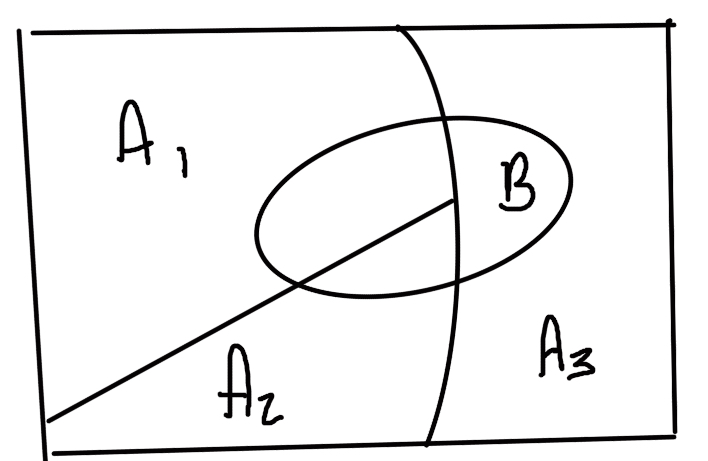
\includegraphics[width=5cm, height=4cm]{images/L02/total_prob.jpeg}
\caption{Total Probability}
\end{figure}

\begin{align}
P(B)=P(A_1)P(B|A_1) + P(A_2)P(B|A_2) + P(A_3)P(B|A_3) = 1
\end{align}
\myequations{Total Probability Theorem}

\subsection{Bayes Rule}

\begin{align}
P(A_i|B) = \frac{P(A_i \cap B)}{P(B)} = \frac{P(A_i)P(B|A_i)}{P(B)} = \frac{P(A_i)P(B|A_i)}{\sum_j P(A_j)P(B|A_j)}
\end{align}
\myequations{Bayes' Rule}

$P(A_j)$ - prior probabilities
